Una volta individuato l'assetto del satellite, occorre un sistema di controllo
che faccia sì che il satellite assuma la posizione e l'assetto desiderati,
attraverso degli attuatori.
Gli attuatori utilizzati per generare forze e coppie sono i propulsori, il cui
funzionamento consiste nell'espellere della massa, detta zavorra.
Essi sono divisi in tre categorie:
\begin{itemize}
  \item a gas freddo: sono costituiti da un contenitore che espelle gas
  \item a propulsione chimica: sia liquida che solida, l'energia è interna al
  propellente
  \item a propulsione elettrica: l'energia si ottiene generando degli ioni, che
  vengono poi accelerati da un campo elettrico
\end{itemize}
Consideriamo un satellite di massa $m$, che all'istante di tempo $t$ abbia
velocità ${\bf v}$ e ipotizziamo che al tempo $t+\Delta t$ sia stata espulsa
$\Delta m$ massa di propellente alla velocità ${\bf u}$. Scriviamo l'equazione
di Newton della quantità di moto
\begin{equation}
(m-\Delta m)({\bf v}+\Delta{\bf v})+\Delta m{\bf u}-m{\bf v}=\Delta t\sum_k F_k
\label{eq:quantita_moto}
\end{equation}
dove $F_k$ rappresenta le forze esterne.
Dividendo l'equazione \ref{eq:quantita_moto} per $\Delta t$, passando al limite
per $\Delta t\rightarrow 0$ e omettendo i termini superiori al primo ordine,
otteniamo
\begin{equation}
m\frac{d{\bf v}}{dt}=\frac{dm}{dt}({\bf v-u})+\sum_k F_k
\end{equation}
ponendo \[ {\bf v_r}={\bf u-v} \] e definendo la spinta come
\begin{equation}
{\bf F}_t=-\frac{dm}{dt}{\bf v}_r=-\dot{m}{\bf v}_r=-\sum_{k=1}^m
\dot{m}_k{\bf v}_{rk}
\label{eq:spinta}
\end{equation}
otteniamo l'equazione
\begin{equation}
m(t)\dot{\bf v}(t)={\bf F}_t+\sum_k F_k
\label{eq:risposta_attuatori}
\end{equation}
Il propellente è conservato ad alta pressione, quindi alla sua espulsione
abbiamo una variazione di pressione da tenere in considerazione e aggiungere
all'equazione \ref{eq:spinta}
\begin{equation}
{\bf F}_t=-\dot{m}{\bf v}_r+A_e(P_e-P_o)=-\dot{m}{\bf v}_e
\end{equation}
Se integriamo la risposta libera, ovvero l'equazione \ref{eq:risposta_attuatori}
senza considerare le forze esterne, otteniamo l'equazione di Tsiolkovsky, che ci
permette di calcolare la massa di prepellente espulso $\Delta m$ per generare
una variazione di velocità $\Delta v$
\begin{equation}
\Delta m=m_0\frac{\Delta v}{v_e}
\end{equation}
dove $m_0$ è la massa iniziale del combustibile. Definiamo, infine, l'impulso
specifico $I_{sp}$ come \[ I_{sp}=\frac{v_e}{g_0}[s] \]

Un propulsore è costituito principalmente da una camera di combustione e da un
ugello, vedi figura \ref{fig:propulsore}. La funzione primaria dell'ugello è di
dirigere e accelerare il combustibile in espulsione. La velocità di espulsione
$v_e$ si calcola dall'equazione dei ges ideali e si dimostra essere
\begin{equation}
v_e=\sqrt{2\frac{\theta_cR}{M}\frac{k}{k-1}\left(1-\left(\frac{P_e}{P_c}\right)^{\frac{k-1}{k}}\right)}
\end{equation}
dove:
\begin{itemize}
  \item $\theta_c$ è la temperatura del propellente
  \item $M$ [kg/kmol] è il peso molecolare del propellente
  \item $k=c_p/c_v$ è il rapporto dei calori specifici a pressione e volume
  costante
  \item $P_c$ e $P_e$ sono, rispettivamente, la pressione della camera di
  combustione e la pressione di uscita dall'ugello
\end{itemize}

\begin{figure}[htp]
\begin{center}
  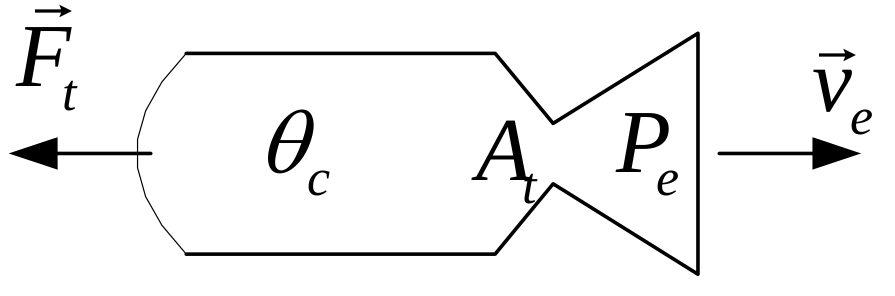
\includegraphics[width=9cm]{modelling/attitude_kinematics_and_dynamics/image/propulsore.png}
  \caption{Schema di un propulsore}
  \label{fig:propulsore}
\end{center}
\end{figure}

I propulsori generano una spinta lungo un vettore velocità ${\bf v}_t$
attraverso un punto di applicazione $a_t$, vedi figura
\ref{fig:geom_propulsore}.
Consideriamo $m$ propulsori, ognuno dei quali genera una spinta diversa per il
satellite, è possibile definire
\begin{equation}
{\bf F}_t=\begin{bmatrix}
{\bf v}_{t,0} & {\bf v}_{t,1} & \dotsb & {\bf v}_{t,m-1}
\end{bmatrix} \begin{bmatrix}
{\bf u}_{t,0} \\ {\bf u}_{t,1} \\ \dotsb \\ {\bf u}_{t,m-1}
\end{bmatrix}={\bf V}_t{\bf u}_t
\label{eq:prop_forza}
\end{equation}
e la coppia
\begin{equation}
{\bf M}_t=\begin{bmatrix}
{\bf a}_{t,0}\times{\bf v}_{t,0} & {\bf a}_{t,1}\times{\bf v}_{t,1} &
\dotsb & {\bf a}_{t,m-1}\times{\bf v}_{t,m-1}
\end{bmatrix} {\bf u}_t= C_t {\bf u_t}
\end{equation}

\begin{figure}[htp]
\begin{center}
  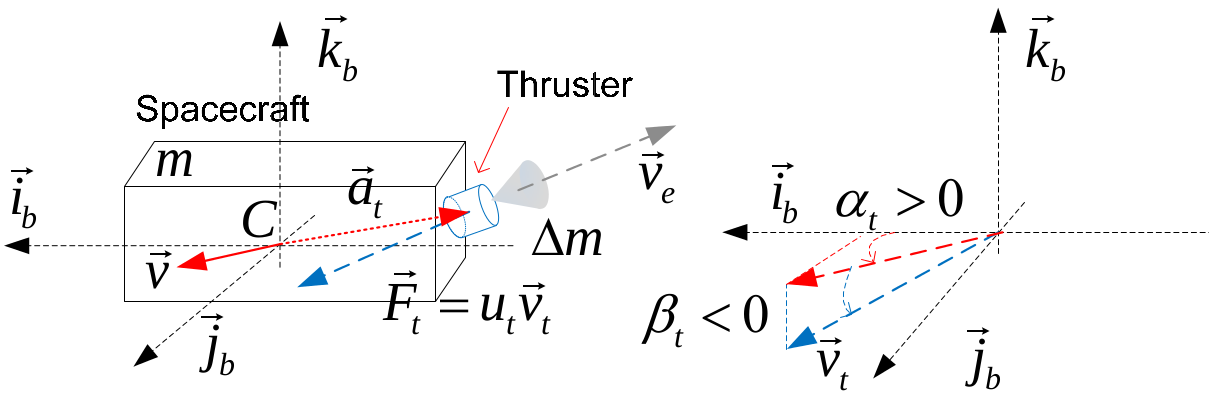
\includegraphics[width=\textwidth]
  {modelling/attitude_kinematics_and_dynamics/image/geometria_del_propulsore.png}
  \caption{Geometria di un propulsore}
  \label{fig:geom_propulsore}
\end{center}
\end{figure}

Resta da definire il posizionamento (dispatching) dei propulsori, dall'equazione
\ref{eq:prop_forza} ricaviamo
\begin{equation}
{\bf u}_t={\bf V}_t^{-1}{\bf F}_t
\end{equation}
La quale ci impone che le direzioni delle spinte siano linearmente indipendenti.

Infine l'ultimo fattore da tenere in considerazione è che i propulsori non
possono generare spinte negative, quindi bisogna disporli a coppia lungo una
direzione in verso opposto, così ogni propulsore può annullare la spinta del
propulsore opposto. Adesso possiamo definire la disposizione finale dei
propulsori come mostrato in figura

\begin{figure}[htp]
\begin{center}
  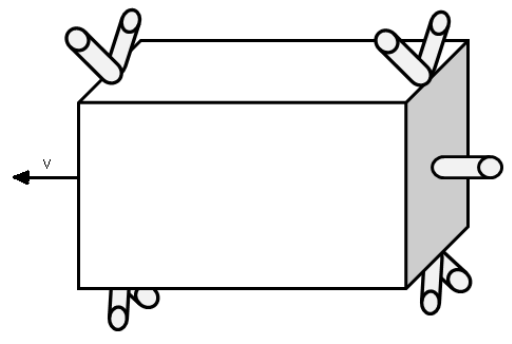
\includegraphics[width=9cm]
  {modelling/attitude_kinematics_and_dynamics/image/dispatching.png}
  \caption{Dispatching dei propulsori}
  \label{fig:dispatching}
\end{center}
\end{figure}

Vengono utilizzati nove propulsore, otto disposti in coppia, e uno, quello
principale, che sarà il propulsore che produrra la spinta maggiore, posizionato
in coda, lungo la direzione di $\vec{v}$, la velocità lineare del satellite.